\documentclass[a4paper,14pt]{article}

\usepackage{comment} % Para comentar várias linhas ao mesmo tempo

%matemática
\usepackage{amsmath}
\usepackage{amssymb}

%diagramação
\usepackage{extsizes}
\everymath{\displaystyle}
\usepackage{geometry}
\usepackage{fancyhdr}
\usepackage{multicol}
\usepackage{graphicx}
\usepackage[brazil]{babel}
\usepackage[shortlabels]{enumitem}
\usepackage{cancel}
\usepackage{textcomp}
\usepackage{tcolorbox}

%tabelas
\usepackage{array} % Para melhor formatação de tabelas
\usepackage{longtable}
\usepackage{booktabs}  % Para linhas horizontais mais bonitas
\usepackage{float}   % Para usar o modificador [H]
\usepackage{caption} % Para usar legendas em tabelas
\usepackage{wrapfig} % Para usar tabelas e figuras flutuantes

\begin{comment}
%tikzpicture
\usepackage{tikz}
\usepackage{scalerel}
\usepackage{pict2e}
\usepackage{tkz-euclide}
\usetikzlibrary{calc}
\usetikzlibrary{patterns,arrows.meta}
\usetikzlibrary{shadows}
\usetikzlibrary{external}
\end{comment}
	
%pgfplots
\usepackage{pgfplots}
\pgfplotsset{compat=newest}
\usepgfplotslibrary{statistics}
\usepgfplotslibrary{fillbetween}

%colours
\usepackage{xcolor}



\columnsep=2cm
\hoffset=0cm
\textwidth=8cm
\setlength{\columnseprule}{.1pt}
\setlength{\columnsep}{2cm}
\renewcommand{\headrulewidth}{0pt}
\geometry{top=1in, bottom=1in, left=0.7in, right=0.5in}

\pagestyle{fancy}
\fancyhf{}
\fancyfoot[C]{\thepage}

\begin{document}
	
	\noindent\textbf{6FMA70 - Matemática} 
	
	\begin{center}Traçando paralelas e perpendiculares (Versão estudante)
	\end{center}
	
	\noindent\textbf{Nome:} \underline{\hspace{10cm}}
	\noindent\textbf{Data:} \underline{\hspace{4cm}}
	
	%\section*{Questões de Matemática}
	
	\begin{multicols}{2}
		\noindent Dada uma reta $r$ e um ponto $P \notin r$.
		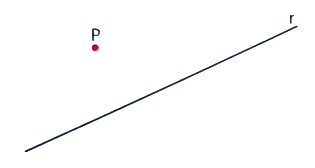
\includegraphics[width=1\linewidth]{6FMA70_imagens/imagem1}
		Para traçar a reta que passa por $P$ e é paralela à reta $r$, fazemos a seguinte construção:
		\begin{itemize}
			\item marcamos um ponto $S$ na reta $r$.
			\item com centro em $S$ e raio $PS$, traçamos o arco (1), achando um ponto $T$ sobre a reta $r$.
			\item com centro em $P$ e mesmo raio, traçamos o arco (2);
			\item com centro em $T$ e mesmo raio, traçamos o arco (3), que encontra o arco (2) em $Q$;
			\item a reta procurada passa pelos pontos $P$ e $Q$.
		\end{itemize}
		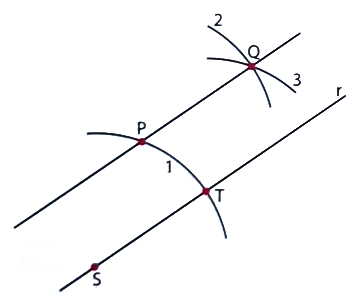
\includegraphics[width=1\linewidth]{6FMA70_imagens/imagem2}
		Para traçar a reta que passa por $P$ e é perpendicular à reta $r$, fazemos a seguinte construção:
		\begin{itemize}
			\item com centro em $P$ e abertura suficiente, traçamos um arco cortando a reta $r$ em dois pontos distintos $M$ e $N$;
			\item com centro nos pontos $M$ e $N$ e mesma abertura, traçamos dois arcos que se cortam em $Q$;
			\item a reta procurada passa pelos pontos $P$ e $Q$.
		\end{itemize}
		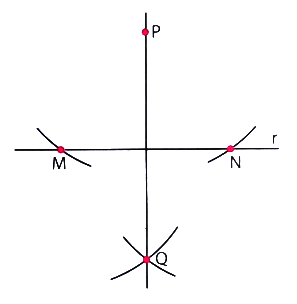
\includegraphics[width=1\linewidth]{6FMA70_imagens/imagem3}
	\end{multicols}
	\noindent\textsubscript{-----------------------------------------------------------------------------------------------------------------------------------------------------------}
    \begin{multicols}{2}
    	\begin{enumerate}
   			\item Usando régua e esquadro, desenhe 5 retas paralelas distintas. \\\\\\\\\\\\\\\\
   			\item Com régua e compasso, trace pelo ponto $X$ retas paralelas às duas retas desenhadas, $m$ e $n$. \\
   			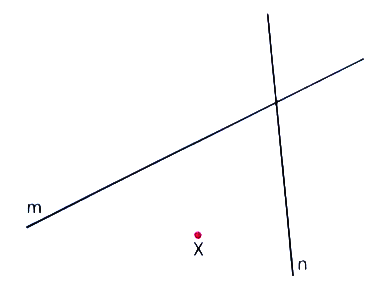
\includegraphics[width=1\linewidth]{6FMA70_imagens/imagem4} \\
   			\item Na figura a seguir, com régua e compasso, trace uma reta $r$ que seja paralela à reta $t$ e que passe pelo ponto $A$. Em seguida, também com régua e compasso, trace uma reta $s$ perpendicular a $r$ e que passe pelo ponto $B$. \\
   			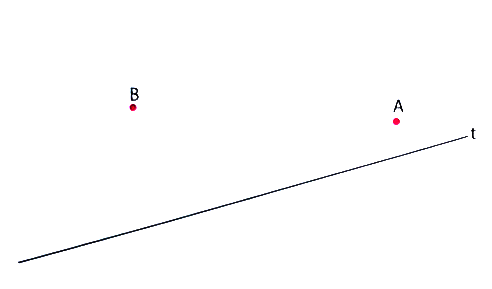
\includegraphics[width=1\linewidth]{6FMA70_imagens/imagem5} \\
   			\item Desenhe, com régua e compasso, a reta perpendicular à reta dada, $t$, pelo ponto $K$ dessa reta. \\
   			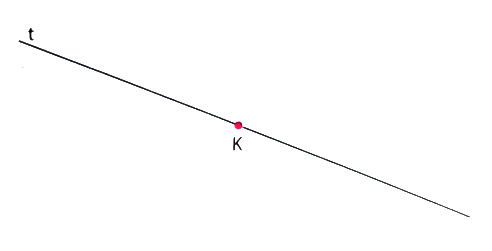
\includegraphics[width=1\linewidth]{6FMA70_imagens/imagem6} \\
   			\textbf{Desafio olímpico} \\\\
   			(OBMEP) Juntando, sem sobreposição, quatro ladrilhos retangulares de 10 cm por 45 cm e um ladrilho quadrado de lado 20 cm, Rodrigo montou a figura abaixo. Com uma caneta vermelha ele traçou o contorno da figura. Qual é o comprimento desse contorno? \\
   			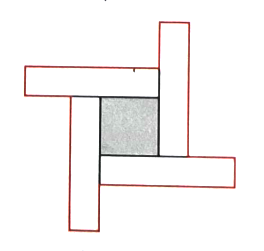
\includegraphics[width=1\linewidth]{6FMA70_imagens/imagem7} \\
   			\begin{enumerate}[a)]
   				\item 180 cm
   				\item 200 cm
   				\item 220 cm
   				\item 280 cm
   				\item 300 cm
   			\end{enumerate}
   			\item Trace por $A$ e por $B$ retas perpendiculares à reta $r$, usando régua e compasso. \\
   			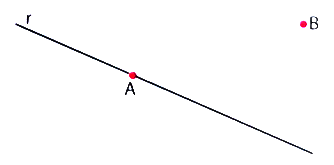
\includegraphics[width=1\linewidth]{6FMA70_imagens/imagem8} \\
   			\item Trace uma reta paralela à reta $r$ que passe pelo ponto $P$ e uma reta perpendicular à reta $r$ que passe pelo ponto $Q$. \\
   			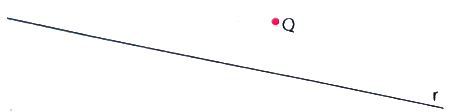
\includegraphics[width=1\linewidth]{6FMA70_imagens/imagem9} \\
   			\item Seja $r$ uma reta e $P \in r$. Trace uma reta perpendicular a $r$, passando por $P$.
	    \end{enumerate} 
        $~$ \\ $~$ \\ $~$ \\ $~$ \\ $~$ \\ $~$ \\ $~$ \\ $~$ \\ $~$ \\ $~$ \\ $~$ \\ $~$ \\ $~$  \\ $~$ \\ $~$ \\ $~$ \\ $~$ \\ $~$ \\ $~$ \\ $~$ \\ $~$ \\ $~$ \\ $~$ \\ $~$ \\ $~$ \\ $~$ \\ $~$ \\ $~$ \\ $~$
	\end{multicols}
\end{document}